\section{evaluation}
\label{sec:evaluation}

To validate the effectiveness of cloud-based burst buffers, 
we conduct several evaluations and simulations in the Amazon EC2 public cloud.
For compute nodes, the burst buffer nodes, and the metadata server, 
we use Amazon EC2 instances shown in Table~\ref{evaluation:amazon_environment}.
All the compute nodes, burst buffer nodes and metadata server node connects with
interconnection network inside Amazon EC2 in the region.

\begin{table}[h]
\centering
\begin{tabular}{|c|c|}
\hline
\cellcolor{lightgray} Region				&		Tokyo		\\
\hline
\cellcolor{lightgray} Instance Type		&		m3.xlarge	\\
\hline
\cellcolor{lightgray} vCPUs				&		4			\\
\hline
\cellcolor{lightgray} ECUs				&		13			\\
\hline
\cellcolor{lightgray} Memory				&		15GiB		\\
\hline
\cellcolor{lightgray} Instance Storage	&		2*40GB(SSD)	\\
\hline
\cellcolor{lightgray} Network Performance	&		High		\\
\hline
\end{tabular}
\caption{evaluation environment}
\label{evaluation:amazon_environment}
\end{table}

% \begin{table}[th]
% \centering
% \begin{tabular}{|c|p{150pt}|}
% \hline
% CPU					&		Intel\textregistered Core\texttrademark i7-3770K CPU @ 3.50GHz\\\hline
% Memory				&		16GB\\\hline
% Storage				&		Crucial m4 CT256M4SSD3 (256GB, mSATA)(Peak read: 500 MB/s, Peak write:260MB/s)*8\\\hline
% RAID Card 			&		Adaptec ASR-7805Q Single\\\hline
% RAID				&		Raid 0\\
% \hline
% \end{tabular}
% \caption{storage environment}
% \label{evaluation:storage_environment}
% \end{table}

Here, vCPUs means the number of virtual CPUs in the instance, 
and a single ECU~(Amazon EC2 Compute Unit) provides the equivalent CPU capacity
of a 1.0-1.2GHz 2007 Opteron or 2007 Xeon processor \cite{AMAZON_AWS}.
For the shared cloud storage, we use Amazon S3 mounted by s3fs\cite{S3FS}.

\subsection{I/O Performance of A Single Compute Node}

\begin{figure}
\centering
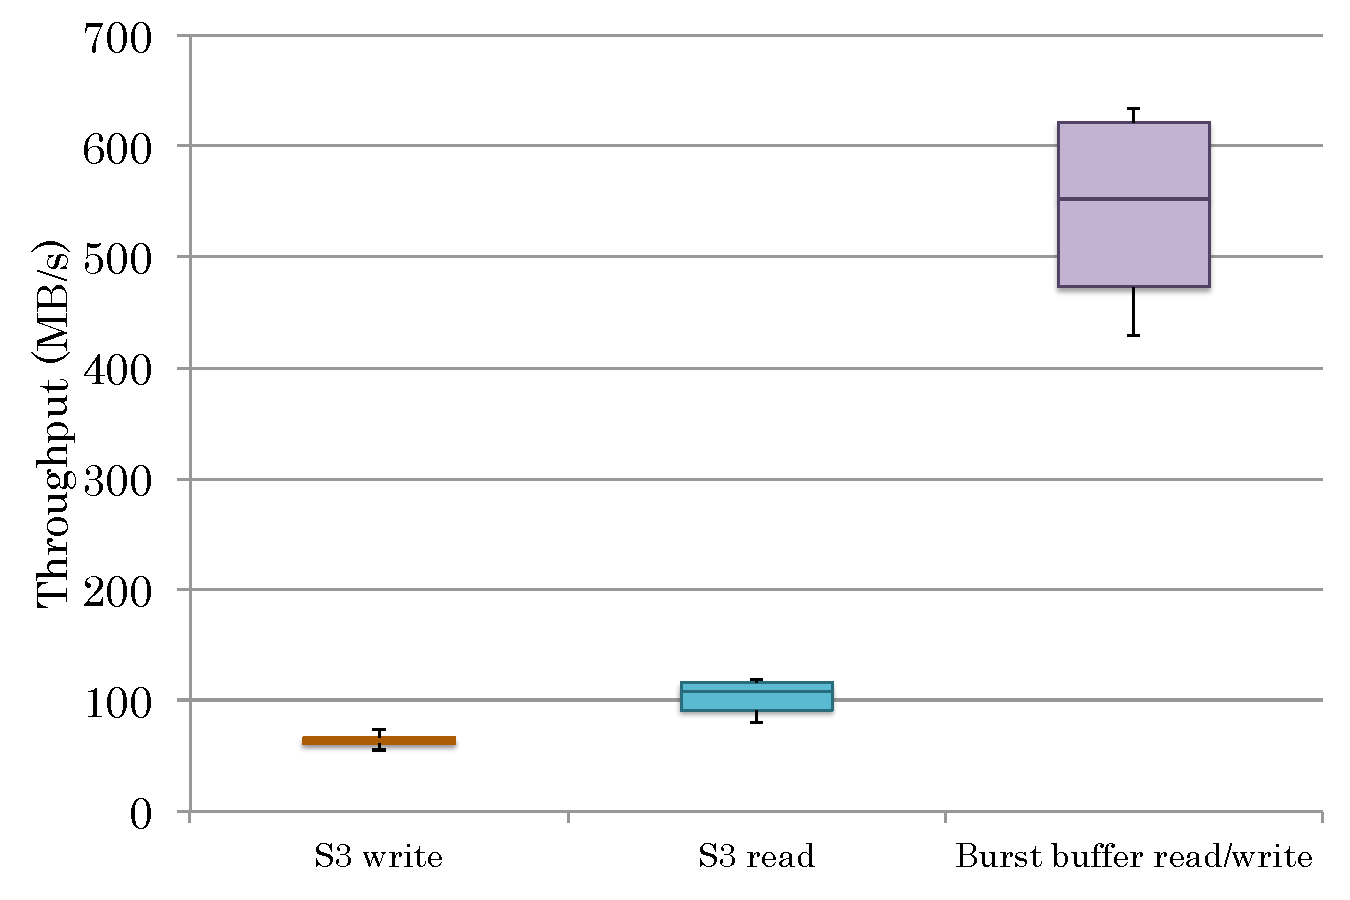
\includegraphics[width=8.5cm]{img/one_client-2.pdf}
\caption{One User Performance}
\label{evaluation:one user performance}
\end{figure}
To illustrate how much our cloud-based burst buffer system will improve I/O
performance of a single compute node, we evaluate the I/O performance when a
single compute node access to our system.
Figure~\ref{evaluation:one user performance} shows sequential read and write
throughputs when a single compute node access to the burst buffers, and S3
under increasing number of burst buffer nodes. All I/O data are distributed
across all burst buffer nodes.

As shown in the figure, by using the cloud-based burst buffer, we can 
achieve 550MB/s for both read and write.
When we read data from burst buffers, data is sent from burst buffers to compute
nodes, and vice versa in writing data. Thus, the both performances are identical
and shown in the single bar. On the other, we can see that applications
can only achieve as 100MB/s for read, and 65MB/s for write without our
cloud-based burst buffers. By using our cloud-based burst buffers, 
we can remarkebly increase performance of I/O having temporal
locality.

\subsection{Scalability of The Cloud-based Burst Buffers}

\begin{figure}
\centering
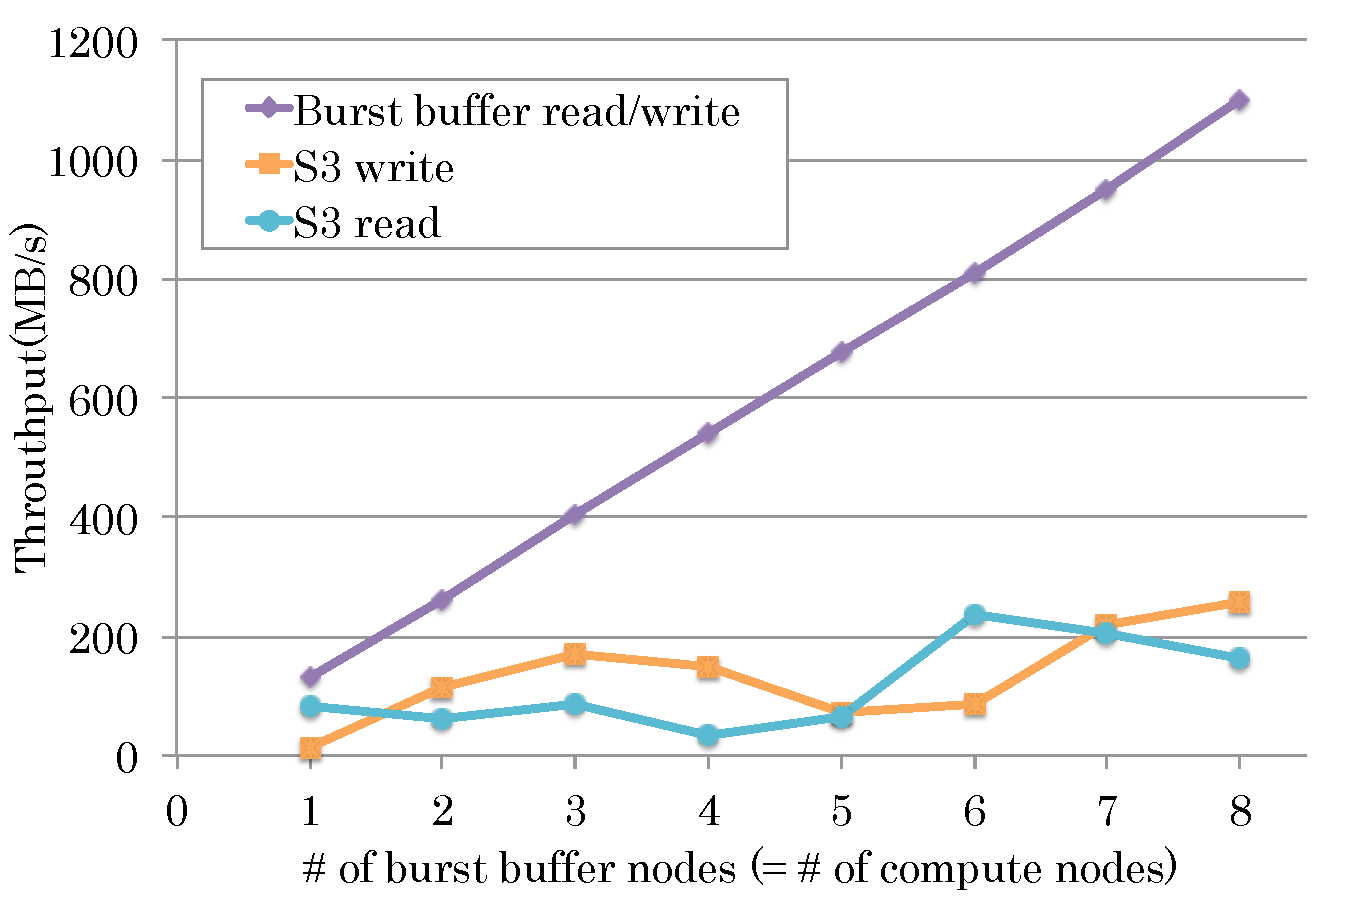
\includegraphics[width=8.5cm]{img/multiple_client-2.pdf}
\caption{Multiple User Performance}
\label{evaluation:multiple user performance}
\end{figure}
Next, we evaluate the scalability of the
cloud-based buffer buffers by increasing both compute nodes and burst
buffer nodes.
Figure~\ref{evaluation:multiple user performance} shows the aggregated
I/O throughput of each method. In this experiment, the number of compute nodes
and burst buffer nodes are same, and each client independently
access each burst buffer node, and one burst buffer node store all the I/O
data for a client.

First we see the result of traditional I/O in which all compute nodes
accesses to S3 concurrently.
However, since the bandwidth of the shared cloud storage is limited, the
overall throughput does not scale well. On the other hands, our system is fairly
scalable because the total bandwidth grows as the burst buffer nodes increase.
%  Then, we found thatng our system.
% Since all the data are stored on the shared storage, and need to
% be transferred via Internet, the read throughput doesn't change by using I/O nodes.
% However when we look at the write throughput, it shows a strong scalability, and achieved 7 times
% improvement with only 4 I/O nodes.

\subsection{Simulation of Real Applications}


\begin{table}
\centering
\begin{tabular}{|c|c|c|c|}
\hline
% 						&	Montage		&		Pov Ray		&		Supernovae		\\\hline
% total I/O size (MB)		&	2132.437508	&		748.916378	&		5203.214882		\\\hline
% total read size(MB)		&	1558.082295	&		681.081228	&		3283.723596		\\\hline
% total write size(MB)	&	574.355213	&		67.83515	&		1919.491286		\\\hline
% read locality size(MB)	&	1500.107713	&		678.155227	&		2429.888509	
% \\\hline compute time (s)		&	18.680705	&		1150.97979	&		1351.987268		\\
\rowcolor{darkgray} 						&	Montage		&		POV-Ray		&		Supernovae		\\\hline
\cellcolor{lightgray} Total I/O size (GB)	&	2.13	&		0.749	&		5.20		\\\hline
 \cellcolor{lightgray}Total read size(GB)	&	1.56	&		0.681	&		3.28		\\\hline
 \cellcolor{lightgray}Total write size(GB)	&	0.574	&		0.067	&		1.92		\\\hline
 \cellcolor{lightgray}Temporal I/O locality size(GB)	&	2.07	&		0.745	&		4.35	
 \\\hline \cellcolor{lightgray}Compute time (s)		&	18.7	&		1151.0	&	
 1352.0		\\
\hline
\end{tabular}
\caption{Applications Execution detail}
\label{evaluation:application execution detail}
\end{table}


\begin{figure}
\centering
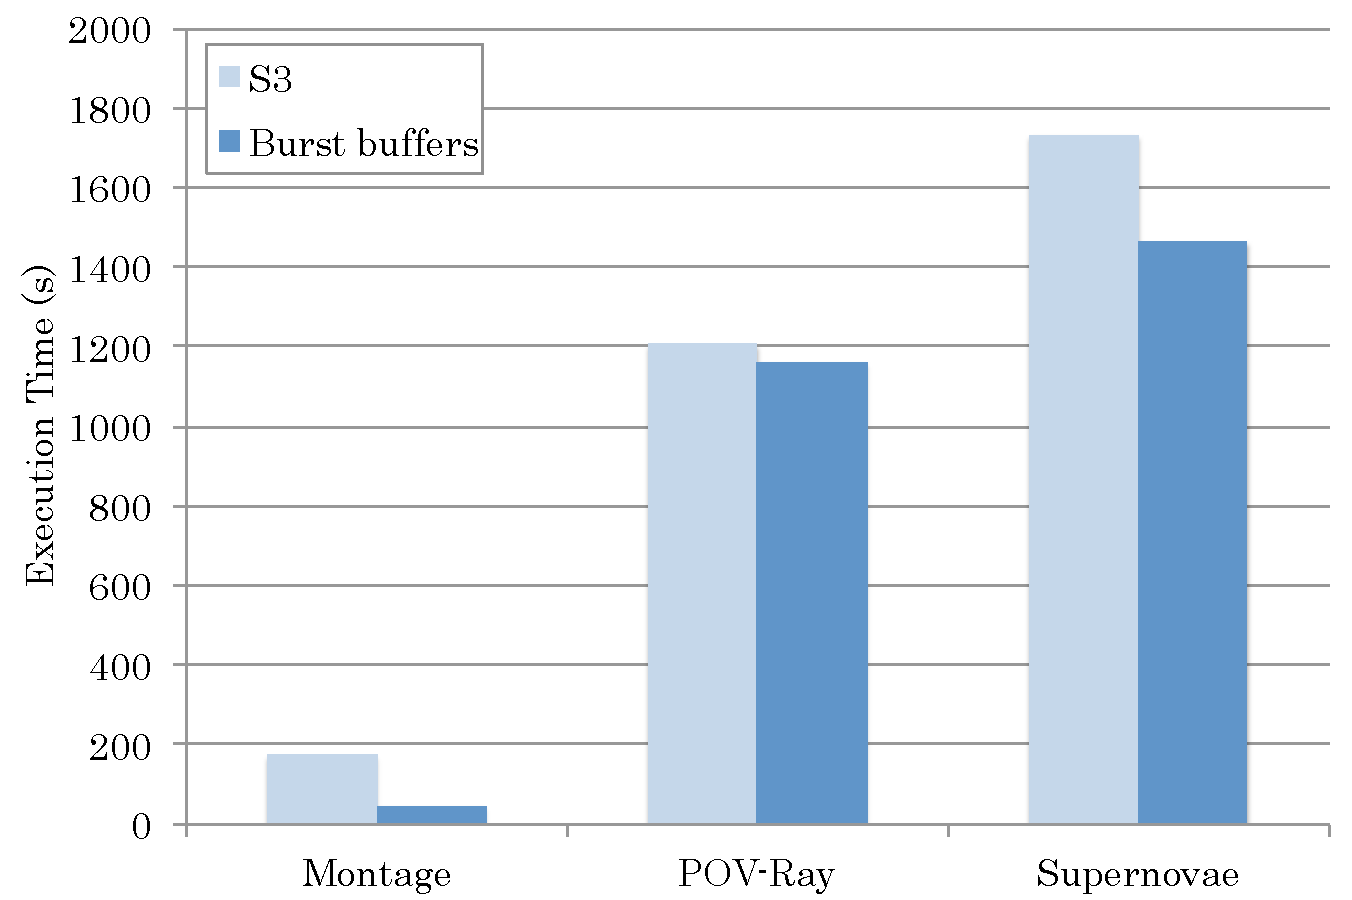
\includegraphics[width=8.5cm]{img/workflows}
\caption{Simulations: Execution times of real applications}
\label{evaluation:simulation result montage}
\end{figure}

 In this section, we simulate the execution of the three applications shown in
 Table.~\ref{background:work flow applications} on our prototype system.
 Since the I/O from other compute nodes will affect the I/O throughput of a
 compute node, we simulate the execution targeting a real cloud environment by
 using the model shown in Section \ref{sec:modeling}.
 In this simulation, we use 8 burst buffer nodes, as well as 8 compute nodes,
 and compute the I/O throughput achieved by one compute node based on the model.
 Figure~\ref{evaluation:simulation result montage} shows the simulation results
 of three real applications on one compute node with 8 burst buffer nodes, and
 other 7 compute nodes. 
 %Figure~\ref{evaluation:simulation result montage} also shows a simulation
 % result of the execution of the three applications on one compute node on Amazon S3 without using burst buffer nodes, and
 %affected by other 7 compute nodes.
 
 As shown in the figure, we  can see that Montage achieves a great speed up by
 using our proposal system, however the other two applications, POV-Ray and
 Supernovae only achieve a little speed up.
 The reason is can be found from Table~\ref{evaluation:application execution detail}.
 From Table~\ref{evaluation:application execution detail}, we can see that Montage has a different
 characteristic compared to the other two applications.
 As we mentioned before, our proposal system can burst applications which have a largest I/O data
 size, so Montage achieves a large speed up on our proposal system, up to 2.9
 times.
 On the contrary, POV-Ray has a heavy computation but a small I/O size, so it
 can only achieve a small speed up.
 In Supernovae case, although the I/O time is reduced by using our proposal system, compare to the
 computation time, the speed up is still small.
 However, because our cloud-based burst buffers accelerate I/O having temporal
 locality, the I/O performance itself remarkably is improved as shown in Figure
 \ref{evaluation:one user performance} and \ref{evaluation:multiple user
 performance}.
 
 \begin{figure}
\centering
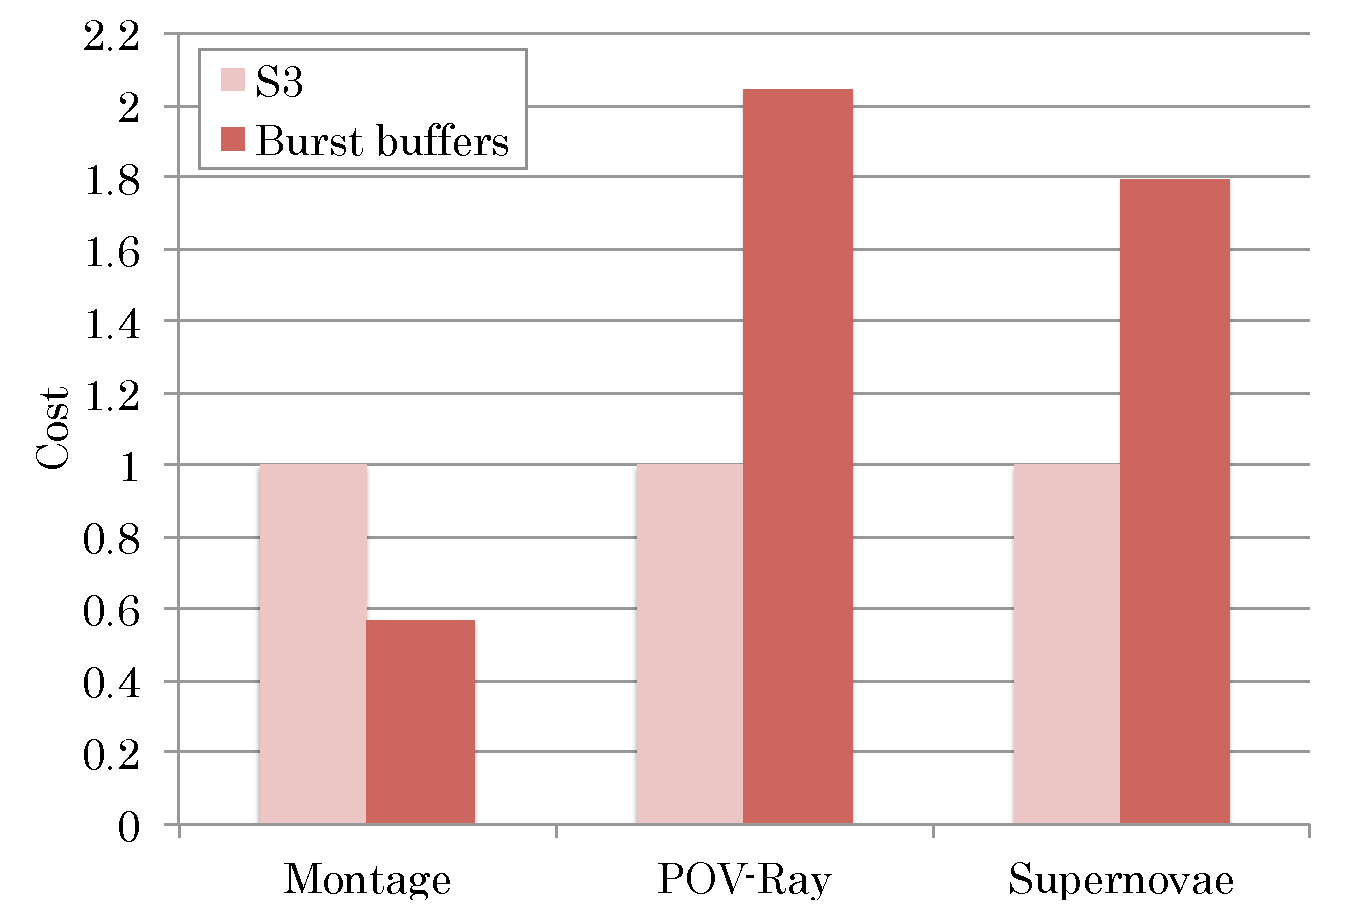
\includegraphics[width=8.5cm]{img/cost-2}
\caption{Simulations: Monetary cost for the executions}
\label{evaluation:simulation result cost}
\end{figure}
 
In addition, we found that if the temporal I/O locality is high as in Montage,
the monetary cost is also improved.
Figure \ref{evaluation:simulation result cost} shows the relative monetary cost
for the execution when the cost of execution without burst buffers, $S3$, is 1.
The estimated costs are computed based on our cost modes in Section
\ref{ssec:cost_model}. As shown in the figure, for Montage, 
we can achieve more that 2 times of saving of the monetary cost in addition to
the I/O performance. Although, the environment with burst buffers use twice
numbers of the Amazone EC2 instances, i.e., additional 8 burst buffers to 8
compute nodes, the execution is cost effective because the execution time can be
reduced by more than two times with our cloud-based burst buffers.
On the other hand, the costs of POV-Ray and Supernovae does not improved. 
This is because these applications conduct much more computation rather than I/O
operations.
If we can dynamically change the number of burst buffers during execution
depending on I/O time and the computation time, then we
can increase the I/O throughput while minimizing the monetary cost. In addition, if we dynamically
change I/O destinations between burst buffers and S3, we can optimize both I/O
throughput and the monetary cost depending on types of applications.
If we analysis the I/O patterns based on MUSE, and optimize the workloads. We
will consider the I/O tuning in future work.

% First we make several assumptions:
% \begin{itemize}
%   \item Master distribute I/O data of applications over all I/O nodes evenly, and applications
%   evenly access I/O data.
% %  \item All I/O data are evenly distributed over all I/O nodes.
% %  \item Applications access all data evenly.
%   \item The I/O bandwidth between compute nodes and I/O nodes is always $T$.
%   \item If multiple compute nodes connect to a single I/O node, they can share the bandwidth of the
%   I/O node equally.
% %  \item Multiple compute nodes can share the throughput of I/O nodes equally.
% \end{itemize}
% 
% As we assume that multiple compute nodes can share the throughput of I/O nodes equally, one
% compute node can achieve $\frac{1}{i+1}$ of the total throughput of I/O node when shared with other
% $i$ compute node, so we can sum it up and get the final throughput:
% \begin{equation}
% \text{Throughput}=\sum_{i=0}^{n-1} \frac{\text{rate}_i}{i+1} \times T
% %\text{T}=\frac{T}{e} 
% %e=1+\frac{n-1}{m}
% \end{equation}
% 
% With above assumptions, then we can calculate the rate of one compute node shared one I/O node with
% other $i$ compute node with total $m$ I/O nodes and $n$ compute node as
% 
% \begin{equation}
% \text{rate}_i=\frac{\dbinom{n-1}{i}(m-1)^{n-i-1}}{m^{n-1}}
% \end{equation}


%Figure.~\ref{evaluation:simulation throughput} shows the one compute node throughput with 8 I/O
%nodes for different number of compute nodes, since for buffered file, compute nodes can assess
% these files from I/O nodes, the read and write throughput are both equal to I/O nodes throughput.
%Since we buffer all the output data, there is only read case can access to unbuffered file which
%can only achieve a low throughput.

%Table~.\ref{evaluation:application execution detail} shows the execution detail of the three
%applications.


% \begin{figure}
% \centering
% 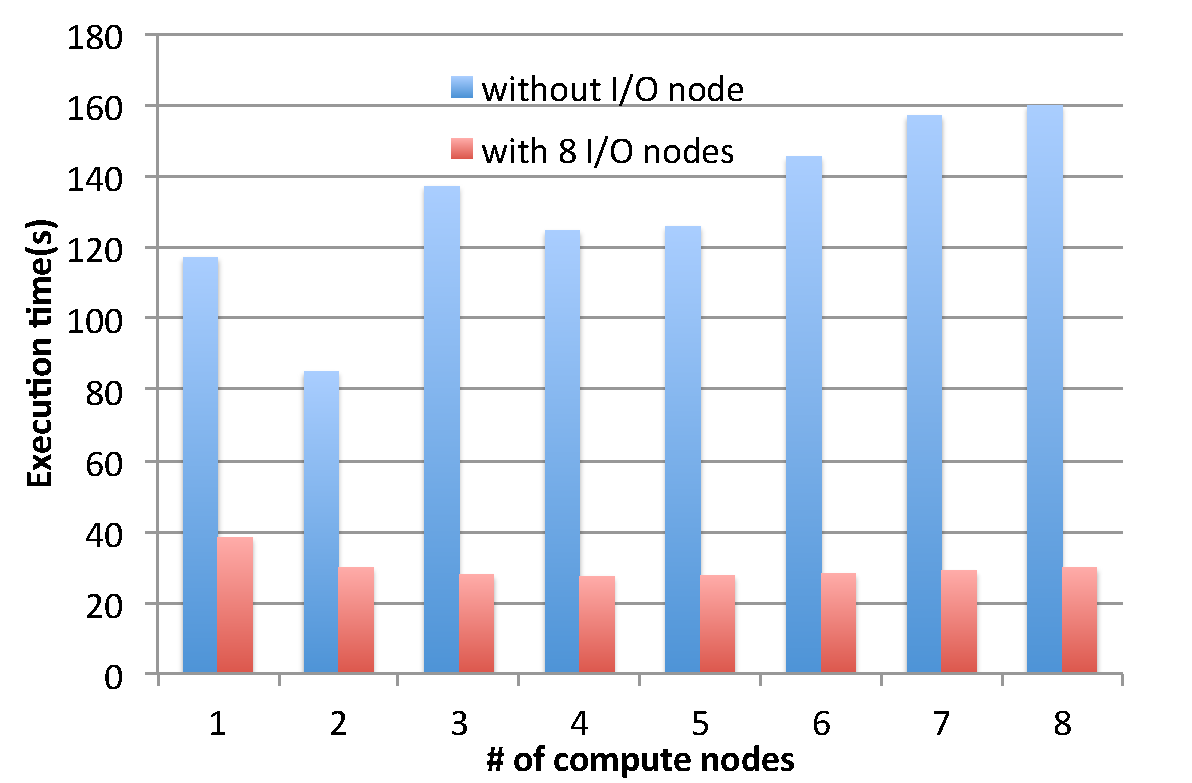
\includegraphics[width=8cm]{img/simulation_montage}
% \caption{simulation result of montage}
% \label{evaluation:simulation result montage}
% \end{figure}
% 
% 
% \begin{figure}
% \centering
% 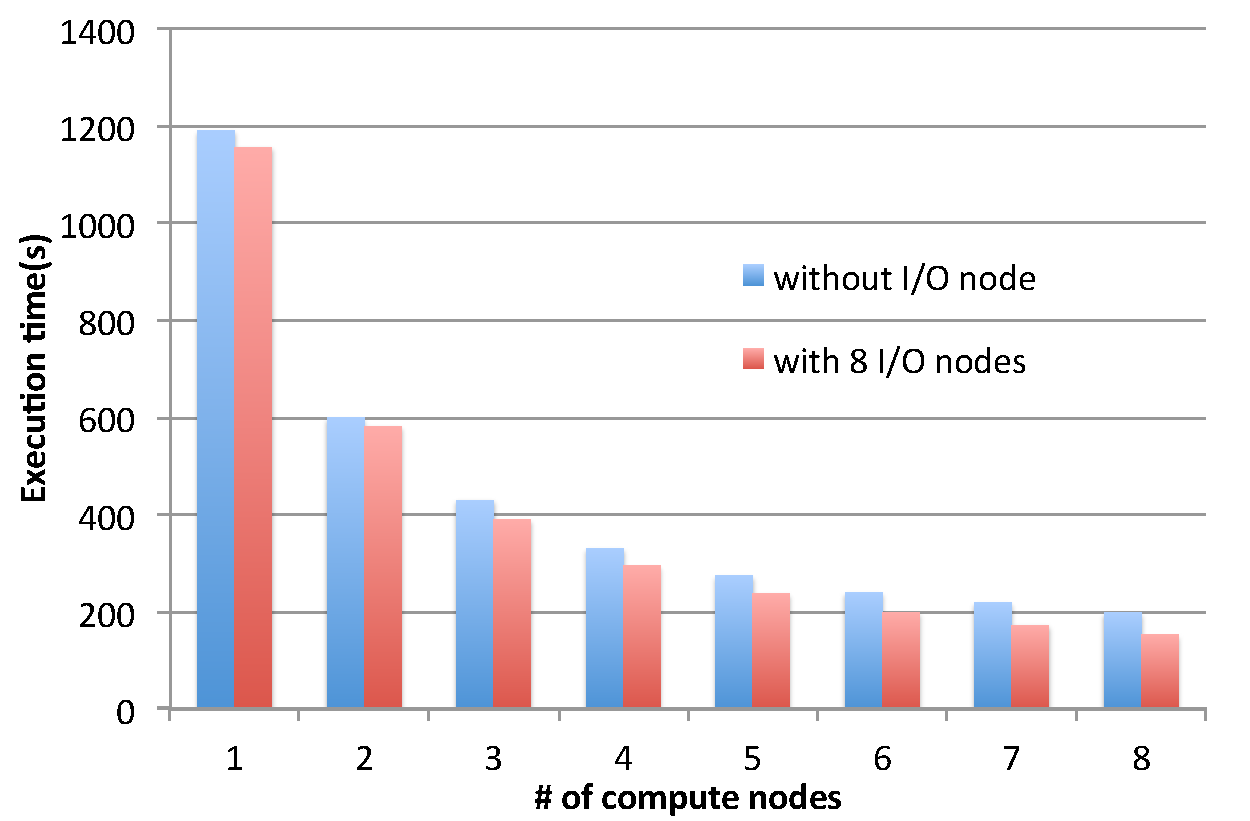
\includegraphics[width=8cm]{img/simulation_povray}
% \caption{simulation result of pov ray}
% \label{evaluation:simulation result pov ray}
% \end{figure}
% 
% \begin{figure}
% \centering
% 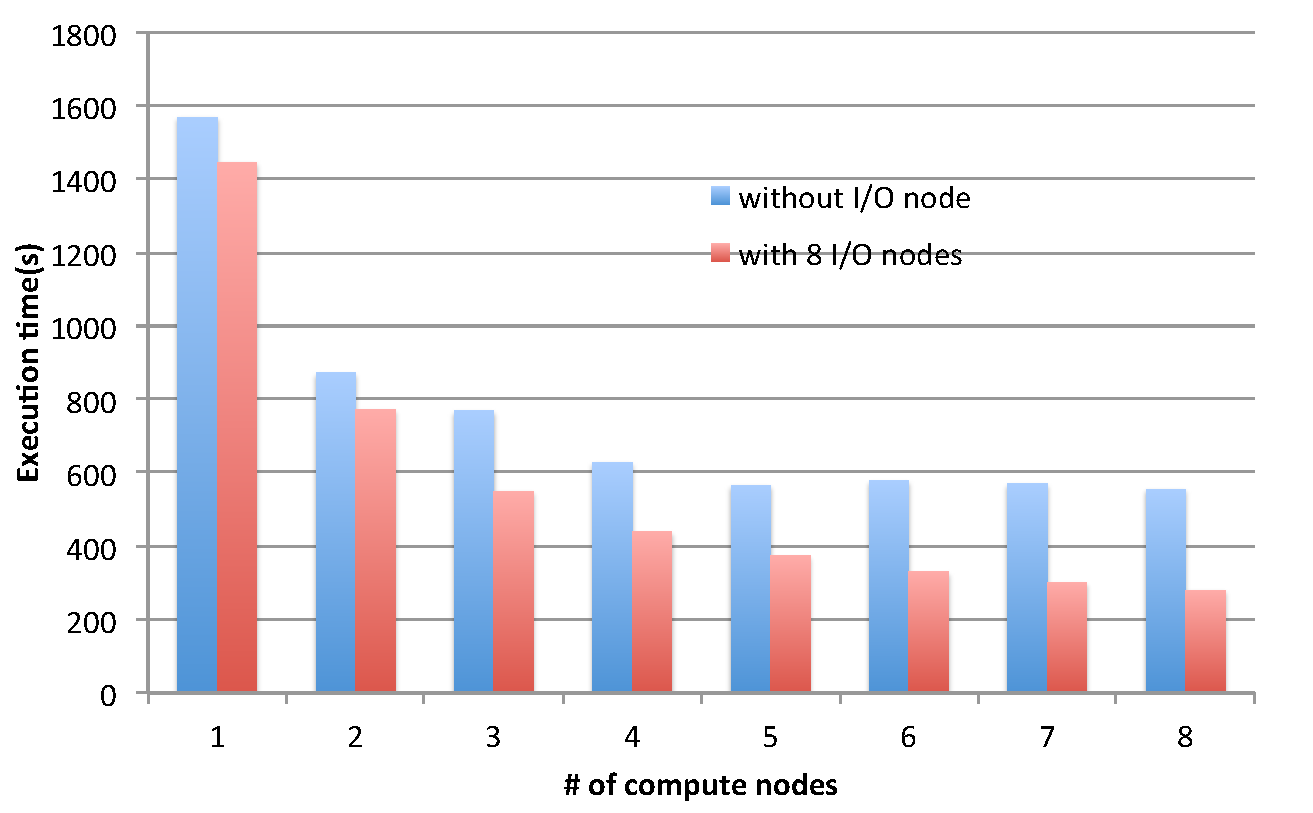
\includegraphics[width=8cm]{img/simulation_supernovae}
% \caption{simulation result of supernovae}
% \label{evaluation:simulation result supernovae}
% \end{figure}

%As we can see from Figure.~\ref{evaluation:simulation result montage},\ref{evaluation:simulation
%result pov ray},\ref{evaluation:simulation result supernovae}, by using our system, all three
%%applications achieved a high improvement.
%Among them, Montage has the largest improvement since it I/O a lot but do not do much
%computation.
%On the contrary, Pov Ray has a heavy computation, and a small I/O size, and gets a small
% performance improvement by using our system.
